% vim:autoindent:set textwidth=78:

% \section{Working with Projections}\label{label_projections}
\section{Utiliser les projections}\label{label_projections}
% \index{Projections!working with}
\index{Projections!utiliser les}

% when the revision of a section has been finalized, 
% comment out the following line:
%\updatedisclaimer

% QGIS allows users to define a global and project-wide CRS (Coordinate
% Reference System) for layers without a pre-defined CRS. It also allows the
% user to define custom coordinate reference systems and supports on-the-fly
% (OTF) projection of vector layers. All these features allow the user to
% display layers with different CRS and have them overlay properly.
QGIS vous permet de d\'efinir une projection (CRS ou Syst\`eme de coordonn\'ees de
r\'ef\'erence) globale et pour des couches qui n'ont pas de projection
pr\'ed\'efinie au niveau du projet. Il permet \'egalement \`a l'utilisateur de d\'efinir
des syst\`emes de coordonn\'ees de r\'ef\'erence personnalis\'es et g\`ere la reprojection
\`a la vol\'ee de couches vectorielles. Toutes ces fonctionnalit\'es permettent \`a
l'utilisateur d'afficher des couches avec diff\'erentes projections et de les
superposer correctement.

% \subsection{Overview of Projection Support}\label{label_projoverview}
\subsection{Aper\c{c}u de la gestion des projections}\label{label_projoverview}

% QGIS has support for approximately 2,700 known CRS. Definitions for 
% each of these CRS are stored in a SQLite database that is installed with
% QGIS. Normally you do not need to manipulate the database directly. In fact,
% doing so may cause projection support to fail. Custom CRS are stored in a
% user database. See Section \ref{sec:customprojections} for
% information on managing your custom coordinate reference systems.
QGIS g\`ere approximativement 2 700 projections connues. Les d\'efinitions pour
chacune d'entre elles sont stock\'ees dans une base de donn\'ees SQLite qui est
install\'ee avec QGIS. Normalement vous n'avez pas besoin de manipuler cette base de
donn\'ees directement. En fait, cela peut poser des probl\`emes de
gestion de projections. Les projections personnalis\'ees y sont stock\'ees dans une
base de donn\'ees utilisateur. Voir la section \ref{sec:customprojections} pour
avoir des informations sur la gestion de vos syst\`emes de coordonn\'ees de
r\'ef\'erence personnalis\'ees.

% The CRS available in QGIS are based on those defined by
% EPSG\index{EPSG} and are largely abstracted from the spatial\_references 
% table in PostGIS\index{PostGIS} version 1.x. The EPSG identifiers are
% present in the database and can be used to specify a CRS in QGIS.
Les projections disponibles dans QGIS sont bas\'ees sur celle d\'efinie par
EPSG\index{EPSG} et sont en grande partie extraite de la table
spatial\_references dans PostGIS\index{PostGIS} version 1.x. Les identifiants
EPSG sont pr\'esents dans la base de donn\'ees et peuvent \^etre utilis\'es pour d\'efinir
une projection dans QGIS.

% In order to use OTF projection, your data must contain information about its
% coordinate reference system or you have to define a global, layer or
% project-wide CRS. For PostGIS layers QGIS uses the spatial reference
% identifier that was specified when the layer was created. For data supported
% by OGR, QGIS relies on the presence of a format specific means of specifying
% the CRS. In the case of shapefiles, this means a file containing the Well
% Known Text (WKT)\index{WKT} specification of the CRS. The projection file
% has the same base name as the shapefile and a prj extension. For example, a
% shapefile named \filename{alaska.shp} would have a corresponding projection
% file named \filename{alaska.prj}.
Dans le but d'utiliser des projections \`a la vol\'ee, vos donn\'ees doivent contenir
des informations sur leurs syst\`emes de coordonn\'ees de r\'ef\'erence ou vous devez
d\'efinir une projection pour votre projet, couche ou globale. Pour les couches
PostGIS, QGIS utilise l'identifiant de r\'ef\'erence spatiale qui a \'et\'e d\'efinie
quand la couche a \'et\'e cr\'e\'ee. Pour les donn\'ees g\'er\'ees par OGR, QGIS utilise un
moyen sp\'ecifique au format de d\'efinition de la projection. Dans le cas de
shapefile, cela signifie un fichier contenant une sp\'ecification Well Known Text
(WKT)\index{WKT} de la projection. Le fichier de projection a le m\^eme nom que
le fichier shape et une extension prj. Par exemple, un shapefile nomm\'e
\filename{alaska.shp} aura un fichier de projection correspondant nomm\'e
\filename{alaska.prj}.

% \subsection{Specifying a Projection}
\subsection{D\'efinir une projection}
% \index{Projections!specifying}
\index{Projections!d\'efinition}
\label{sec:projection-specifying}

% QGIS no longer sets the map CRS to the coordinate reference system of the
% first layer loaded. When you start a QGIS session with layers that do not
% have a CRS, you need to control and define the CRS definition for these
% layers. This can be done globally or project-wide in the \tab{CRS} tab under
% \mainmenuopt{Settings} > \dropmenuopttwo{mActionOptions}{Options} (See
% Figure~\ref{fig:crsdialog}).
QGIS ne d\'efinit plus la projection de la carte au syst\`eme de
coordonn\'ees de r\'ef\'erence de la premi\`ere couche charg\'ee. Lorsque vous d\'emarrez
une session QGIS avec des couches qui ne poss\`edent pas de projection, vous devez
contr\^oler et d\'efinir la d\'efinition de la projection pour ces couches. Cela peut
\^etre r\'ealis\'ee globalement ou par projet dans l'onglet \tab{projection} dans 
\mainmenuopt{Pr\'ef\'erences} > \dropmenuopttwo{mActionOptions}{Options} (voir
 Figure~\ref{fig:crsdialog}).

\begin{itemize}
% \item \checkbox{Prompt for CRS}
\item \checkbox{Demande de projection}
% \item \checkbox{Project wide default CRS will be used}
\item \checkbox{La valeur par d\'efaut au niveau du projet sera utilis\'ee}
% \item \checkbox{Global default CRS displayed below will be used}
\item \checkbox{La valeur globale par d\'efaut affich\'e ci-dessous sera
utilis\'ee}
\end{itemize}

% The global default CRS \texttt{proj=longlat +ellps=WGS84 +datum=WGS84
% +no\_defs} comes predefined in QGIS but can of course be changed, and the new
% definition will be saved for subsequent QGIS sessions.    
La projection globale par d\'efaut \texttt{proj=longlat +ellps=WGS84 +datum=WGS84
 +no\_defs} est pr\'ed\'efinie dans QGIS mais peut bien sur \^etre chang\'ee, et la
nouvelle d\'efinition sera sauv\'ee pour les prochaines sessions de QGIS.

\begin{figure}[ht]
   \begin{center}
%    \caption{CRS tab in the QGIS Options Dialog
% \nixcaption}\label{fig:crsdialog}\smallskip
   \caption{Onglet Projection dans la bo\^ite de dialogue de QGIS
\nixcaption}\label{fig:crsdialog}\smallskip
   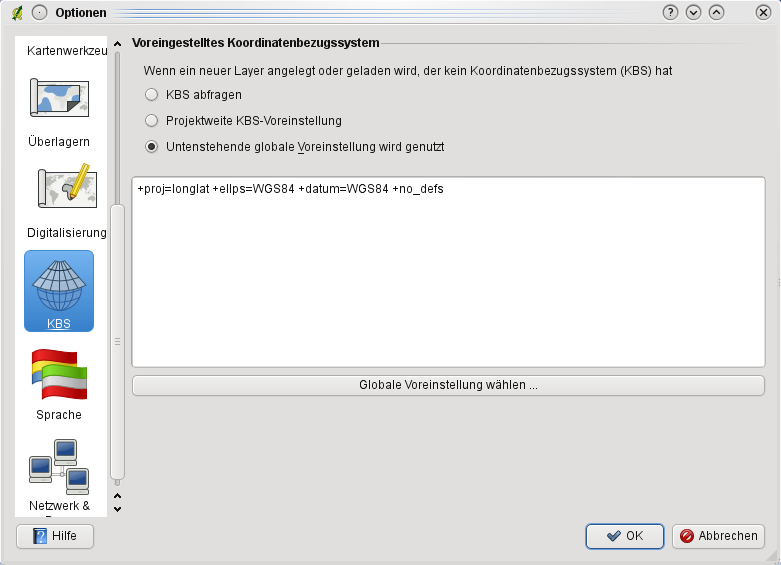
\includegraphics[clip=true, width=12cm]{crsdialog}
\end{center}
\end{figure}

% If you want to define the coordinate reference system for a certain layer
% without CRS information, you can also do that in the \tab{General} tab of the
% raster properties (\ref{label_generaltab}) and vector properties
% (\ref{vectorgeneraltab}) dialog. If your layer already has a CRS defined, it
% will be displayed as shown in Figure~\ref{fig:vector_symbology}.
Si vous voulez d\'efinir le syst\`eme de coordonn\'ees de r\'ef\'erence pour certaines
couches sans information sur la projection, vous pouvez \'egalement faire cela
dans l'onglet \tab{G\'en\'eral} de la bo\^ite de dialogue propri\'et\'e de la couche
raster (\ref{label_generaltab}) ou de celle de la couche vecteur
(\ref{vectorgeneraltab}). Si votre couche a d\'ej\`a une projection d\'efinie, elle
sera affich\'ee comme montr\'e dans la figure~\ref{fig:vector_symbology}.

% \subsection{Define On The Fly (OTF) Projection}\label{label_projstart}
\subsection{D\'efinir une projection \`a la vol\'ee (OTF)}\label{label_projstart}

% QGIS does not have OTF projection enabled by default, and this function is
% currently only supported for vector layers. To use OTF projection, you must
% open the \dropmenuopttwo{mActionOptions}{Project Properties} dialog, select a
% CRS and activate the \checkbox{Enable on the fly projection} checkbox.
% There are two ways to open the dialog:
QGIS n'active pas la projection \`a la vol\'ee par d\'efaut, et cette fonction est
seulement g\'er\'ee pour les couches vectorielles. Pour utiliser la projection \`a la
vol\'ee, vous devez ouvrir la bo\^ite de dialogue
\dropmenuopttwo{mActionOptions}{Propri\'et\'es du projet}, s\'electionner une
projection et cocher la case \`a cocher \checkbox{Activer la projection \`a la
vol\'ee}. Il y a deux mani\`eres pour ouvrir la bo\^ite de dialogue :

\begin{enumerate}
% \item Select \dropmenuopttwo{mActionOptions}{Project Properties} from the
% \mainmenuopt{Settings} menu.
\item S\'electionnez \dropmenuopttwo{mActionOptions}{Propri\'et\'es du
projet} \`a partir du menu \mainmenuopt{Pr\'ef\'erences}.
% \item Click on the \toolbtntwo{mIconProjectionDisabled}{projector} icon in the
% lower right-hand corner of the statusbar.
\item Cliquez sur l'ic\^one \toolbtntwo{mIconProjectionDisabled}{projection} dans
le coin en base \`a droite de la barre de statut.
\end{enumerate}

% If you have already loaded a layer, and want to enable OTF projection, the
% best practice is to open the \tab{Coordinate Reference System} tab of the
% \dialog{Project Properties} dialog, select the CRS of the currently loaded
% layer, and activate the \checkbox{Enable on the fly projection} checkbox. The
% \toolbtntwo{mIconProjectionEnabled}{projector} icon will show a green hook
% and all subsequently loaded vector layers will be OTF projected to the
% defined CRS.
Si vous avez d\'ej\`a charg\'ee une couche, et d\'esirez activer la projection \`a la
vol\'ee, la meilleure fa\c{c}on de faire est d'ouvrir l'onglet \tab{Syst\`eme de
coordonn\'ees de r\'ef\'erence} de la bo\^ite de dialogue \dialog{Propri\'et\'es du
projet}, s\'electionner la projection de la couche charg\'ee, et d'activer la case
\checkbox{Activer la projection \`a la vol\'ee}. L'ic\^one
\toolbtntwo{mIconProjectionEnabled}{projection} affichera un symbole vert et
toutes les couches vecteurs charg\'ees plus tard seront projet\'ees \`a la vol\'ee dans
la projection d\'efinie.

% The \tab{Coordinate Reference System} tab of the \dialog{Project Properties}
% dialog contains four important components as numbered in Figure
% \ref{fig:projections} and described below.
L'onglet \tab{Syst\`eme de Coordonn\'ees de R\'ef\'erence} de la bo\^ite de dialogue
\dialog{Propri\'et\'es du projet} contient quatre composants importants comme
num\'erot\'e \`a la figure \ref{fig:projections} et d\'ecrit ci-dessous.

\begin{figure}[ht]
   \begin{center}
%    \caption{Projection Dialog \nixcaption}\label{fig:projections}\smallskip
   \caption{Bo\^ite de dialogue
Projection\nixcaption}\label{fig:projections}\smallskip
   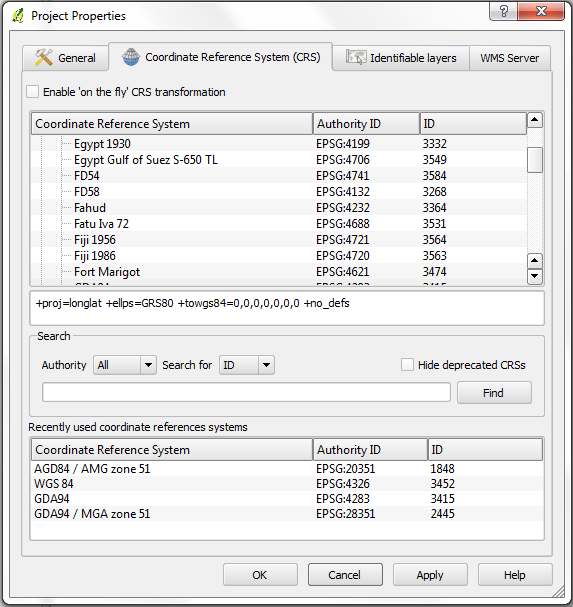
\includegraphics[clip=true, width=12cm]{projectionDialog}
\end{center}
\end{figure}

\begin{enumerate}
% \item \textbf{Enable on the fly projection}\index{Projections!enabling} -
% this checkbox is used to enable or disable OTF projection. When off, each
% layer is drawn using the coordinates as read from the data source. When on,
% the coordinates in each layer are projected to the coordinate reference
% system defined for the map canvas.
\item \textbf{Activer la projection \`a la vol\'ee}\index{Projections!activer} -
cette case \`a cocher est utilis\'ee pour activer ou d\'esactiver la projection \`a la
vol\'ee. Lorsqu'elle ne l'est pas, chaque couche est dessin\'ee en utilisant les
coordonn\'ees lues dans la source de donn\'ees. Lorsqu'elle est activ\'ee, les
coordonn\'ees de chaque couche sont projet\'ees dans le syst\`eme de coordonn\'ees de
r\'ef\'erence d\'efinie pour la carte.
% \item \textbf{Coordinate Reference System} - this is a list of all CRS
% supported by QGIS, including Geographic, Projected and Custom coordinate
% reference systems. To use a CRS, select it from the list by expanding
% the appropriate node and selecting the CRS. The active CRS is preselected.
\item \textbf{Syst\`eme de Coordonn\'ees de R\'ef\'erence} - c'est une liste de toutes
les projections g\'er\'ees par QGIS, incluant les syst\`emes de coordonn\'ees
de r\'ef\'erence g\'eographiques, projet\'ees et personnalis\'ees. Pour utiliser une
projection, s\'electionnez-la dans la liste en d\'eroulant le noeud appropri\'e et en
s\'electionnant la projection. La projection active est pr\'es\'electionn\'ee.
% \item \textbf{Proj4 text} - this is the CRS string used by the Proj4
% projection engine. This text is read-only and provided for informational
% purposes.
\item \textbf{Texte Proj4} - c'est une cha\^ine de projection utilis\'e par le
moteur de projection Proj4. Ce texte est en lecture seul et est fournit pour
information.
% \item \textbf{Search} - if you know the EPSG identifier or the name 
% for a Coordinate Reference System, you can use the search feature to find it.
% Enter the identifier and click on \button{Find}.
\item \textbf{Rechercher} - si vous connaissez le code EPSG ou le nom d'un
syst\`eme de coordonn\'ees de r\'ef\'erence, vous pouvez utiliser la fonction
rechercher pour le retrouver. Entrez le code et cliquez sur le bouton
\button{Trouver}.
\end{enumerate}

\begin{Astuce}
%  \caption{\textsc{Project Properties Dialog}}
 \caption{\textsc{bo\^ite de dialogue Propri\'et\'e du projet}}
\qgistip{
% If you open the \dialog{Project Properties} dialog from the
% \mainmenuopt{Settings} menu, you must click on the \tab{Coordinate Reference
% System} tab to view the CRS settings. Opening the dialog from the
% \toolbtntwo{mIconProjectionEnabled}{projector} icon will automatically bring
% the \tab{Coordinate Reference System} tab to the front.
Si vous ouvrez la bo\^ite de dialogue \dialog{Propri\'et\'es du projet} \`a partir du
menu \mainmenuopt{Pr\'ef\'erences}, vous devez cliquer sur l'onglet \tab{Syst\`eme de
Coordonn\'ees de R\'ef\'erence} pour voir les d\'efinitions de projection. Ouvrir la
bo\^ite de dialogue \`a partir de l'ic\^one
\toolbtntwo{mIconProjectionEnabled}{projection} vous amenera directement dans
l'onglet \tab{Syst\`eme de Coordonn\'ees de R\'ef\'erence}.
}
\end{Astuce}

% \subsection{Custom Coordinate Reference System}\label{sec:customprojections}
\subsection{Syst\`eme de Coordonn\'ees de R\'ef\'erence
personnalis\'ees}\label{sec:customprojections}
\index{Projections!personnalisation}

% If QGIS does not provide the coordinate reference system you need, you
% can define a custom CRS. To define a CRS, select
% \dropmenuopttwo{mIconNew}{Custom CRS} from the \mainmenuopt{Settings} menu.
% Custom CRS are stored in your QGIS user database. In addition to your custom
% CRS, this database also contains your spatial bookmarks and other custom data.
Si QGIS ne fournit pas le syst\`eme de coordonn\'ees de r\'ef\'erence dont vous avez
besoin, vous pouvez en d\'efinir un. Pour cela, s\'electionnez
\dropmenuopttwo{mIconNew}{Projection personnalis\'ee} \`a partir du menu
\mainmenuopt{Pr\'ef\'erences}. Les projections personnalis\'ees sont stock\'ees dans la
base de donn\'ees utilisateur de QGIS. En plus de votre projection personnalis\'ee,
cette base de donn\'ees contient \'egalement vos signets spatiaux et autres donn\'ees
personnalis\'ees.

\begin{figure}[ht]
   \begin{center}
%    \caption{Custom CRS Dialog
% \nixcaption}\label{fig:customprojections}\smallskip
\caption{Bo\^ite de dialogue Projection
personnalit\'ee\nixcaption}\label{fig:customprojections}\smallskip
   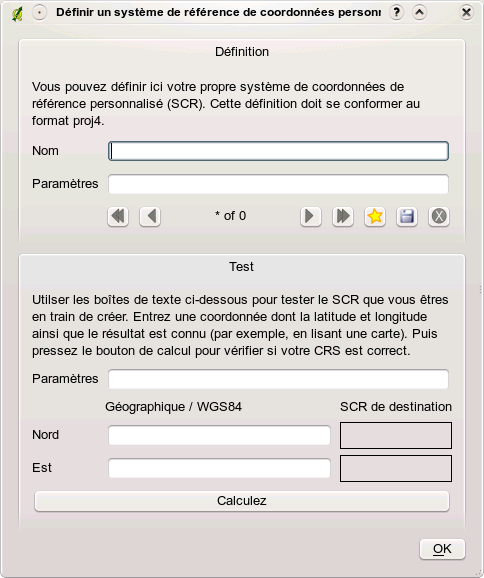
\includegraphics[clip=true, width=12cm]{customProjectionDialog}
\end{center}
\end{figure}

% Defining a custom CRS in QGIS requires a good understanding of the Proj.4
% projection library. To begin, refer to the Cartographic Projection Procedures
% for the UNIX Environment - A User's Manual by Gerald I. Evenden, U.S.
% Geological Survey Open-File Report 90-284, 1990 (available at 
% \url{ftp://ftp.remotesensing.org/proj/OF90-284.pdf}).
D\'efinir une projection personnalis\'ee dans QGIS n\'ecessite une bonne
compr\'ehension de la biblioth\`eque de projection Proj4. Pour commencer, r\'ef\'erez
vous aux Proc\'edures de Projection Cartographique pour l'environnement UNIX - Un
manuel d'utilisateur de Gerald I. Evenden, U.S. Geological Survey Open-File
Report 90-284, 1990 (disponible sur
\url{ftp://ftp.remotesensing.org/proj/OF90-284.pdf}).
% This manual describes the use of the \usertext{proj.4} and related command
% line utilities. The cartographic parameters used with \usertext{proj.4} are
% described in the user manual, and are the same as those used by QGIS.
Ce manuel d\'ecrit l'utilisation de \usertext{proj.4} et les applications en
lignes de commandes li\'ees. Les param\`etres cartographiques utilis\'es avec
\usertext{proj.4} sont d\'ecrit dans le manuel utilisateur et sont les m\^emes que
ceux utilis\'es par QGIS.

% The \dialog{Custom Coordinate Reference System Definition} dialog requires
% only two parameters to define a user CRS:
La bo\^ite de dialogue \dialog{D\'efinition d'un syst\`eme de coordonn\'ees de
r\'ef\'erence personnalis\'ee} n\'ecessite seulement deux param\`etres pour d\'efinir une
projection personnalis\'ee :
\begin{enumerate}
% \item a descriptive name and
\item un nom descriptif et
% \item the cartographic parameters in PROJ.4 format.
\item les param\`etres cartographiques au format PROJ.4.
\end{enumerate}
% To create a new CRS, click the \toolbtntwo{mIconNew}{New} button and enter a
% descriptive name and the CRS parameters. After that you can save your CRS by
% clicking the button \toolbtntwo{mActionFileSave}{Save}.
Pour cr\'eer une nouvelle projection, cliquez sur le bouton
\toolbtntwo{mIconNew}{Nouveau} et entrez un nom descriptif et les param\`etres de
la projection. Apr\`es cela vous pouvez sauver votre projection en cliquant le
bouton  \toolbtntwo{mActionFileSave}{Sauver}.

% Note that the \guilabel{Parameters} must begin with a \usertext{+proj=}-block,
% to represent the new coordinate reference system.
Remarquez que les \guilabel{Param\`etres} doivent d\'ebuter par un
 bloc \usertext{+proj=} pour repr\'esenter le nouveau syst\`eme de coordonn\'ees de
r\'ef\'erence.

% You can test your CRS parameters to see if they give sane results by
% clicking on the \button{Calculate} button inside the \guiheading{Test} block 
% and pasting your CRS parameters into
% the \guilabel{Parameters} field. Then enter known WGS 84 latitude and
% longitude values in \guilabel{North} and \guilabel{East} fields respectively.
% Click on \button{Calculate} and compare the results with the known values in
% your coordinate reference system.
Vous pouvez tester vos param\`etres de projection pour voir s'il donne les m\^emes
r\'esultats en cliquant sur le bouton \button{Calculer} dans le bloc 
\guiheading{Test} et copiant vos param\`etres de projection dans le champ
\guilabel{Param\`etres}. Puis entrez une latitude et longitude connue en WGS 84
dans les champs \guilabel{Nord} et \guilabel{Est} respectivement. Cliquez sur
le bouton \button{Calculer} et comparez les r\'esultats avec les valeurs connues
dans votre syst\`eme de coordonn\'ees de r\'ef\'erence.

